\documentclass{article}

\usepackage{amsmath,amssymb}
\usepackage{array}
\usepackage{geometry}
\usepackage{graphicx}

\geometry{a4paper, margin=2.5cm}

\begin{document}

% ============================================================
\section*{PPO (Proximal Policy Optimization)}

\subsection*{First, a story}

You are a martial artist. After each bout (one rollout), the coach (the advantage function $\hat{A}$) hands you a detailed review: ``the side kick at second 23 should be faster'', ``the defense at second 47 was too conservative''. The report was written \textbf{based on how you fought then} (the old policy $\pi_{\theta_{\text{old}}}$).

You take the report and adjust toward the optimum. It doesn't feel like enough, so you adjust again\ldots\ after $K=20$ rounds you have become a completely different fighter --- yet the coach's advice is still that original report, written about the you of twenty rounds ago. The more you follow it, the stranger your movements become, until you lose disastrously.

\textbf{The core conflict}:
\begin{itemize}
  \item the data was collected by the old policy $\pi_{\theta_\text{old}}$;
  \item each round's update optimizes the new policy $\pi_\theta$;
  \item the more updates, the further apart they drift --- the staler the data.
\end{itemize}

This is the dilemma of unconstrained multi-round policy updates, and the core problem PPO solves:

\[
\boxed{\text{How to update the policy many times, safely, without wasting samples?}}
\]

\subsection*{Formalization}

The policy gradient theorem gives the gradient direction:

\[
\nabla_\theta J(\theta) = \mathbb{E}_{\pi_\theta}\!\left[\nabla_\theta \log \pi_\theta(a_t \mid s_t)\,\hat{A}_t\right]
\]

To reuse data collected by the old policy, introduce the \textbf{importance-sampling weight} (the probability ratio):

\[
\boxed{r_t(\theta) = \frac{\pi_\theta(a_t \mid s_t)}{\pi_{\theta_\text{old}}(a_t \mid s_t)}}
\]

$r_t = 1$ means the new and old policies agree completely at this step; $r_t \gg 1$ or $r_t \ll 1$ means the policy has drifted severely.

Substituting into the surrogate objective:

\[
L^{\text{CPI}}(\theta) = \hat{\mathbb{E}}_t\!\left[r_t(\theta)\,\hat{A}_t\right]
\]

\textbf{In plain words}: multiply each step's advantage $\hat{A}_t$ by ``the ratio of new to old policy'', and optimizing this surrogate repeatedly lets one batch of data be reused many times. \textbf{The problem}: after $K$ rounds $r_t$ can drift far from $1$ --- the surrogate becomes untrustworthy and the gradient direction fails.

% ============================================================
\section*{Why does unconstrained updating collapse?}

\subsection*{The valid range of importance sampling}

Importance sampling implicitly assumes the two distributions are ``close enough''. If $\pi_\theta$ and $\pi_{\theta_\text{old}}$ diverge too much, the estimator's variance explodes:

\[
\operatorname{Var}\!\left[r_t(\theta)\,\hat{A}_t\right] \propto \mathbb{E}\!\left[r_t^2(\theta)\right] - 1
\]

As $r_t$ departs from $1$ (in either direction), the gradient estimate's variance grows sharply and the update direction becomes unreliable.

\subsection*{$K$ rounds of updating drift $r$}

Take clip-free PPO ($K=20$ rounds): after each round $\theta$ changes and $r_t(\theta)$ drifts along:

\begin{itemize}
  \item round 1: $r_t \approx 1$, the gradient estimate is trustworthy;
  \item round 4: $r_t$ starts to drift; the advantage estimate becomes biased;
  \item round 8: $r_t$ is severely off, the advantage estimate fails entirely, the gradient direction is wrong --- training collapses.
\end{itemize}

\begin{figure}[!htbp]
  \centering
  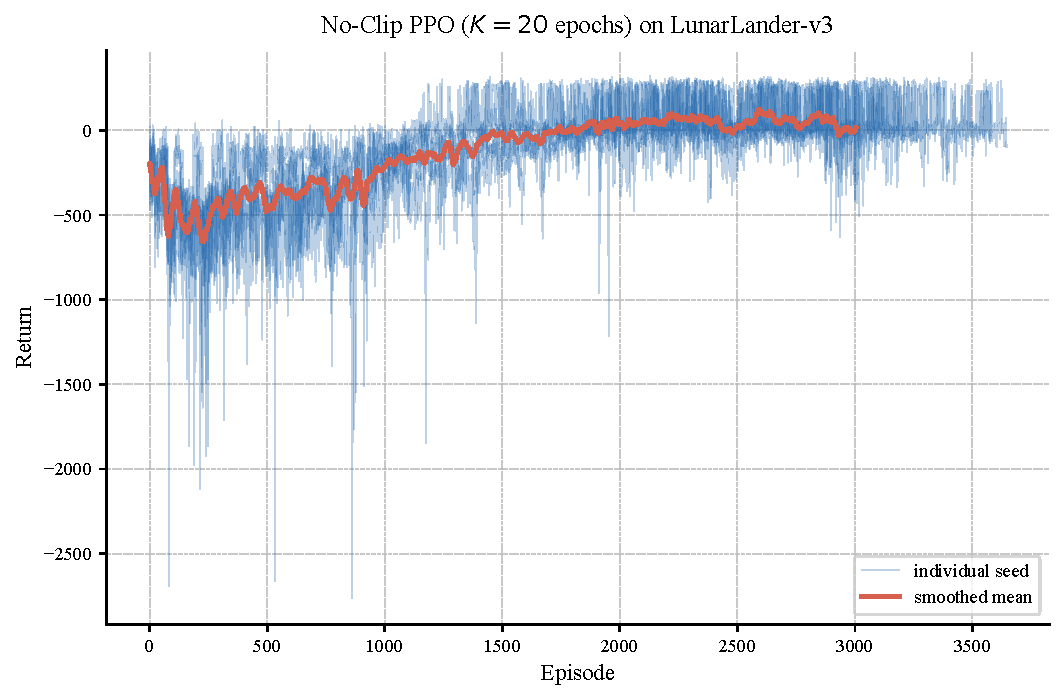
\includegraphics[width=\textwidth]{fig1_noclip_instability.pdf}
  \caption{Clip-free PPO ($K=20$ rounds, mini-batch) on LunarLander-v3, 5 seeds (thin blue lines).
           Some seeds' returns drop to $-8000$ early on (40 times worse than the random policy), then recover slowly.
           The smoothed mean (red) stays below the clipped version throughout training.}
\end{figure}

% ============================================================
\section*{PPO-Clip: the truncated surrogate objective}

\subsection*{The core formula}

PPO's solution is remarkably simple: \textbf{clip $r_t$ to the neighborhood of $[1-\varepsilon,\;1+\varepsilon]$};
beyond the bound, no gradient incentive remains.

\[
\boxed{L^{\text{CLIP}}(\theta)
  = \hat{\mathbb{E}}_t\!\left[\min\!\left(
      r_t(\theta)\,\hat{A}_t,\;
      \operatorname{clip}\!\left(r_t(\theta),\,1-\varepsilon,\,1+\varepsilon\right)\hat{A}_t
    \right)\right]}
\]

$\varepsilon$ is typically $0.2$.

\begin{figure}[!htbp]
  \centering
  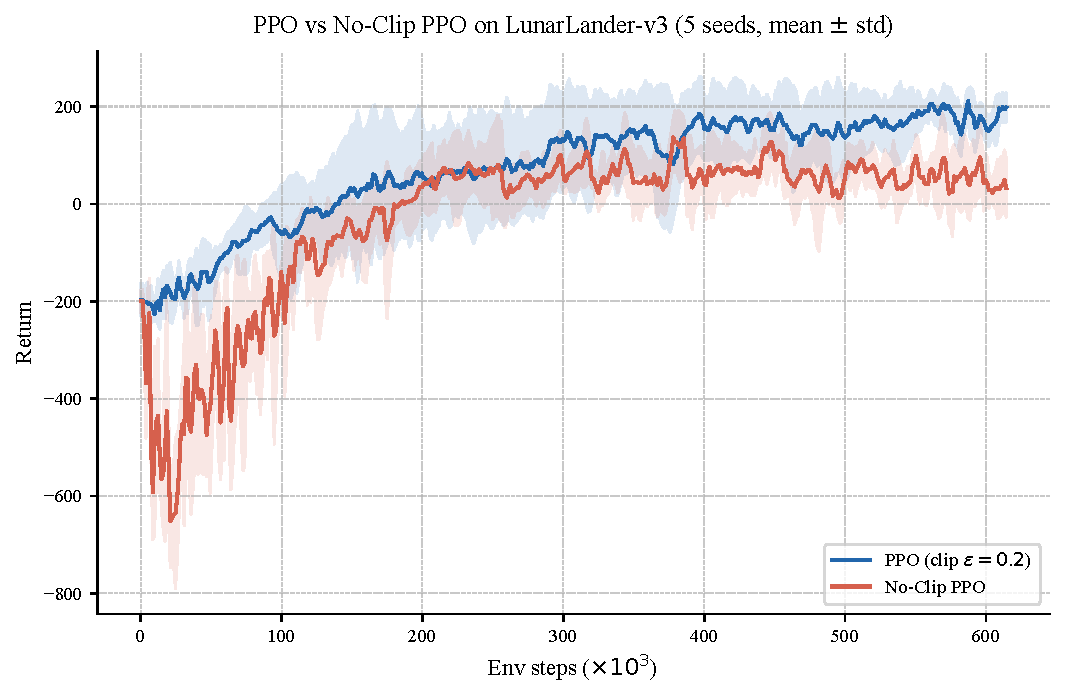
\includegraphics[width=\textwidth]{fig2_clip_vs_noclip.pdf}
  \caption{PPO-Clip (blue) vs.\ clip-free PPO (red) on LunarLander-v3 (5 seeds, mean $\pm$ std).
           The x-axis is environment steps ($\times10^3$); both methods use exactly the same total steps ($300\times2048\approx614$k),
           ruling out the confound that ``a better policy has longer episodes and hence fewer episodes''.
           The clipped version rises steadily, entering positive returns after about 400k steps;
           the clip-free version crashes to $-600\sim-1000$ early, recovers slowly, and never catches up, with larger variance.}
\end{figure}

\subsection*{Intuition: cutting off both extremes}

Read $\min$ in two cases.

\textbf{Case A: $\hat{A}_t > 0$ (this action beat the average; raise its probability)}
\begin{itemize}
  \item $r_t$ rising (the new policy favors this action) $\to$ good, but past $1+\varepsilon$ the clipped value is used and the gradient goes to zero;
  \item \textbf{Core principle}: the policy change is ``already enough'' --- no further pushing.
\end{itemize}

\textbf{Case B: $\hat{A}_t < 0$ (this action was worse; lower its probability)}
\begin{itemize}
  \item $r_t$ falling (the new policy avoids this action) $\to$ good, but below $1-\varepsilon$ the clipped value is used and the gradient goes to zero;
  \item \textbf{Core principle}: as above --- excessive avoidance is no longer rewarded either.
\end{itemize}

\underline{Only updates heading in the favorable direction and not yet past the bound provide gradient drive}.

\subsection*{How the clip suppresses $r$'s drift}

\begin{figure}[!htbp]
  \centering
  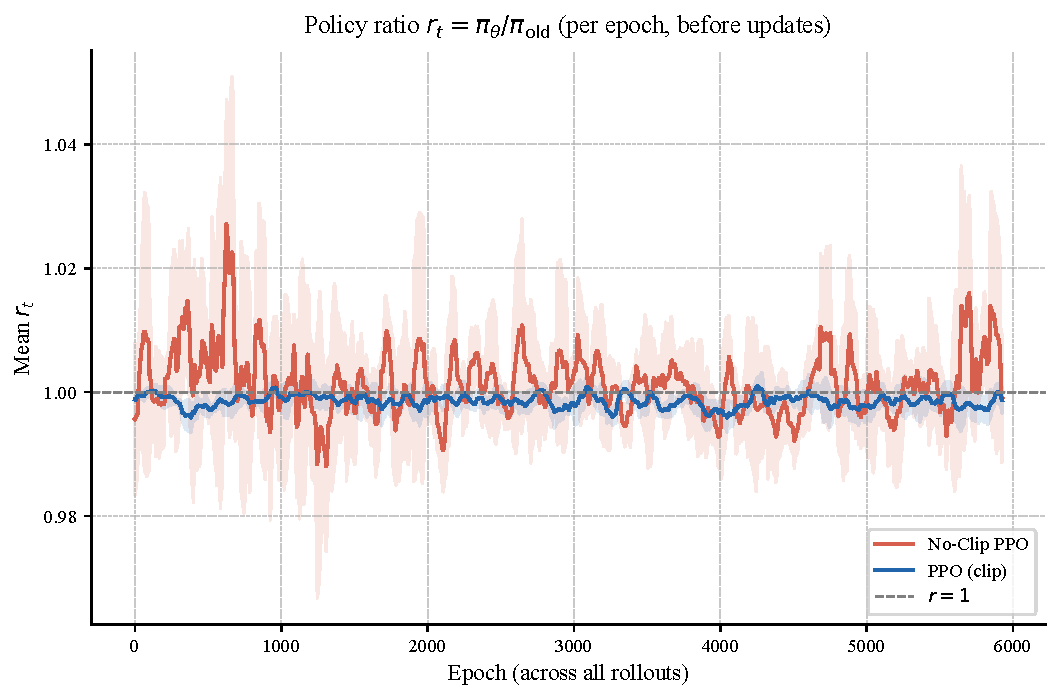
\includegraphics[width=\textwidth]{fig3_policy_ratio.pdf}
  \caption{The batch-mean policy ratio $r_t$, measured on the full batch before each epoch (5 seeds, mean $\pm$ std).
           Clip-free (red) deviates more, reaching $\sim\!1.017$ early; PPO-Clip (blue) stays near $1$.
           Beyond the mean, individual transitions' $r_t$ can far exceed the 1.2 clip bound --- it is exactly these tails being clipped that prevents the accumulation of erroneous gradients.}
\end{figure}

\subsection*{Why does the clip work?}

\begin{enumerate}
  \item \textbf{Suppresses the ``step size'' of each update}: once $r_t$ leaves $[1-\varepsilon, 1+\varepsilon]$, that sample no longer contributes gradient in the direction of further deviation --- drift is \textbf{softly suppressed}, not hard-forbidden; individual $r_t$ may still exceed the bound (see Figure~3);
  \item \textbf{Symmetric protection}: an action's probability can be neither over-increased nor over-decreased;
  \item \textbf{A pessimistic lower bound}: $L^{\text{CLIP}}$ lower-bounds $L^{\text{CPI}}$ and never overstates the improvement --- updates happen only when the improvement is real.
\end{enumerate}

% ============================================================
\section*{Generalized Advantage Estimation (GAE)}

\subsection*{Why GAE}

The advantage function $A(s,a) = Q(s,a) - V(s)$ measures ``how much better than average''. Practice offers two extreme estimators:

\[
\begin{array}{c|c|c}
\text{Estimator} & \text{Bias} & \text{Variance} \\
\hline
\hat{A}^{\text{MC}} = \displaystyle\sum_{l=0}^{\infty}\gamma^l r_{t+l} - V(s_t) & \text{zero} & \text{very large} \\[6pt]
\hat{A}^{\text{TD}} = r_t + \gamma V(s_{t+1}) - V(s_t) & \text{biased} & \text{very small} \\
\end{array}
\]

GAE interpolates between the two, with $\lambda \in [0,1]$ tuning the bias--variance trade-off.

\subsection*{The GAE formula}

Define the TD residual (one-step temporal-difference error):
\[
\delta_t^V = r_t + \gamma V(s_{t+1}) - V(s_t)
\]

GAE sums exponentially weighted multi-step TD residuals:

\[
\boxed{\hat{A}_t^{\text{GAE}(\gamma,\lambda)} = \sum_{l=0}^{\infty}(\gamma\lambda)^l\,\delta_{t+l}^V}
\]

The equivalent recursion (used in implementations, inducting backwards from the end):

\[
\hat{A}_t = \delta_t^V + \gamma\lambda\,\hat{A}_{t+1}
\]

\subsection*{The meaning of $\lambda$: interpolating between TD and MC}

\[
\begin{array}{c|c|c}
\lambda & \text{degenerates to} & \text{effect} \\
\hline
\lambda = 0 & \hat{A}_t = \delta_t^V \;\;(\text{1-step TD}) & \text{low variance, biased} \\[4pt]
\lambda = 1 & \hat{A}_t = \displaystyle\sum_{l=0}^{\infty}\gamma^l r_{t+l} - V(s_t)\;\;(\text{MC}) & \text{zero bias, high variance} \\[6pt]
\lambda = 0.95 & \text{common in practice} & \text{bias/variance compromise} \\
\end{array}
\]

\textbf{In plain words}: the larger $\lambda$, the more one trusts the actually sampled distant returns rather than the critic's predictions. PPO typically takes $\gamma = 0.99,\;\lambda = 0.95$.

% ============================================================
\section*{The full PPO algorithm}

\subsection*{The total loss}

\[
\boxed{L^{\text{PPO}}(\theta)
  = L^{\text{CLIP}}(\theta)
  \;-\; c_1\,L^{\text{VF}}(\theta)
  \;+\; c_2\,S[\pi_\theta]}
\]

The terms:
\begin{itemize}
  \item $L^{\text{CLIP}}$: the clipped policy-gradient loss (maximized);
  \item $L^{\text{VF}} = \hat{\mathbb{E}}_t\!\left[\left(V_\theta(s_t) - \hat{V}_t^{\,\text{target}}\right)^2\right]$: the critic's squared error (minimized, $c_1 \approx 0.5$);
  \item $S[\pi_\theta] = \hat{\mathbb{E}}_t\!\left[-\sum_a \pi_\theta(a|s_t)\log\pi_\theta(a|s_t)\right]$: the entropy bonus preventing premature policy degeneration (maximized, $c_2 \approx 0.01$).
\end{itemize}

The actor and critic \textbf{share the network parameters} $\theta$; one backpropagation updates both.

\subsection*{The PPO-Clip loop}

\begin{enumerate}
  \item \textbf{Collect a rollout}: run $T$ steps in the environment with $\pi_{\theta_\text{old}}$, recording $(s_t, a_t, r_t, s_{t+1})$;
  \item \textbf{Estimate advantages}: compute $\hat{A}_t$ by GAE; value targets $\hat{V}_t^{\,\text{target}} = \hat{A}_t + V_{\theta_\text{old}}(s_t)$;
  \item \textbf{$K$ epochs of mini-batch updates}:
    \begin{enumerate}
      \item forward pass, compute $r_t(\theta)$ and $L^{\text{PPO}}(\theta)$;
      \item clip gradients ($\|\nabla\theta\|_2 \le 0.5$), backpropagate;
      \item update $\theta$.
    \end{enumerate}
  \item Set $\theta_\text{old} \leftarrow \theta$, return to step 1.
\end{enumerate}

\textbf{Why are $K$ epochs safe now?} Once a sample's $r_t$ leaves $[1-\varepsilon, 1+\varepsilon]$, the clip removes its gradient in the direction of further deviation, suppressing the error accumulation of $K$ epochs on the same batch. Note this is a \textbf{soft constraint}: individual $r_t$ still exceed the bound (Figure~3) --- there is simply no gradient incentive in the deviating direction to amplify them further.

% ============================================================
\section*{PPO vs other policy-gradient methods}

\subsection*{One table to compare}

\begin{center}
\small
\setlength{\tabcolsep}{3pt}
\begin{tabular}{>{\raggedright\arraybackslash}p{0.18\textwidth}|>{\raggedright\arraybackslash}p{0.29\textwidth}|>{\raggedright\arraybackslash}p{0.24\textwidth}|>{\raggedright\arraybackslash}p{0.22\textwidth}}
\textbf{Method} & \textbf{Sample efficiency} & \textbf{Stability} & \textbf{Complexity} \\
\hline
REINFORCE  & very low (one update per batch) & low (high variance) & simplest \\
A2C        & low (same) & medium & simple \\
TRPO       & high (one natural-gradient update per batch) & high (KL constraint) & very complex (second-order) \\
PPO-Clip   & high ($K$ epochs per batch) & high (clip constraint) & simple (first-order) \\
\end{tabular}
\end{center}

\subsection*{Why is PPO more popular than TRPO?}

TRPO (Trust Region Policy Optimization) uses the KL divergence as a hard constraint:

\[
\max_\theta L^{\text{CPI}}(\theta)
\quad \text{s.t.} \quad
\hat{\mathbb{E}}_t\!\left[D_{\text{KL}}\!\left(\pi_{\theta_\text{old}}(\cdot\mid s_t)
  \;\|\; \pi_\theta(\cdot\mid s_t)\right)\right] \le \delta
\]

Theoretically the strictest --- but it requires the natural gradient (inverting the Fisher information matrix), prohibitively expensive on deep networks.

PPO turns the ``trust region'' into a \textbf{soft constraint}: beyond the bound nothing is penalized; it \underline{simply receives no further gradient incentive}.

\begin{itemize}
  \item \textbf{TRPO}: ``cross the line and get punished'' (hard constraint, second-order optimization);
  \item \textbf{PPO}: ``near the line, we stop pushing'' (soft constraint, first-order optimization).
\end{itemize}

Comparable results --- but PPO needs only first-order gradients, is simple and fast, and has become the default baseline among on-policy methods.

% ============================================================
\section*{Where this chapter sits in the RL landscape}

\begin{enumerate}
  \item \textbf{The TD route} $\to$ Q-Learning $\to$ DQN (discrete actions, value-based);
  \item \textbf{The MC route} $\to$ REINFORCE $\to$ policy gradients (high variance, one update per batch);
  \item \textbf{Actor-Critic} $\to$ GAE $\to$ \underline{PPO} (this chapter: low variance + safe multi-epoch updates);
  \item \textbf{Continuous actions / offline settings} $\to$ SAC (maximum-entropy RL) $\to$ offline RL (IQL etc.).
\end{enumerate}

PPO is today's default on-policy baseline --- nearly every RLHF pipeline (LLM alignment) builds on PPO at its core. Given how robust PPO already is, why do continuous-action and offline settings still need their own algorithms?

\subsection*{References}

\begin{enumerate}
  \item Schulman et al.\ (2017). Proximal Policy Optimization Algorithms. \textit{arXiv:1707.06347}.
  \item Schulman et al.\ (2015). Trust Region Policy Optimization. \textit{ICML}.
  \item Schulman et al.\ (2016). High-Dimensional Continuous Control Using Generalized Advantage Estimation. \textit{ICLR}.
  \item Sutton \& Barto (2018). \textit{Reinforcement Learning: An Introduction} (2nd ed.). Chapter 13.
  \item Hands-on RL (Chinese). Chapter 12: the PPO algorithm.
\end{enumerate}

\end{document}
